\documentclass[tikz,convert={outfile=\jobname.svg}]{standalone}

\usetikzlibrary{shapes.misc}

\tikzset{cross/.style={cross out, draw=black, minimum size=2*(#1-\pgflinewidth), inner sep=0pt, outer sep=0pt},
%default radius will be 1pt. 
cross/.default={2.5pt}}

\begin{document}

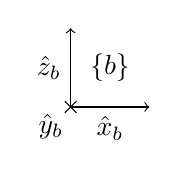
\begin{tikzpicture}
    \draw [->] (0,0) -- (1, 0) node[pos=0.5, below]{$\hat{x}_{b}$};
    \draw [->] (0,0) -- (0, 1) node[pos=0.5, left]{$\hat{z}_{b}$};
    \draw (0,0) node[cross] {};
    \draw (0,0) node[pos=0, xshift=-0.25cm, yshift=-0.25cm]{$\hat{y}_{b}$};
    \draw (0,0) node[pos=0, xshift=0.5cm, yshift=0.5cm]{$\{b\}$};
\end{tikzpicture}

\end{document}